\documentclass[11pt]{article}

\newcommand{\numpy}{{\tt numpy}}    % tt font for numpy

% for symbols
\usepackage{bbold}
\usepackage{amsmath,amssymb}
\DeclareMathOperator*{\argmin}{arg\,min}
\DeclareMathOperator*{\argmax}{arg\,max}
\setlength\parindent{20pt}

% for images
\usepackage{graphicx}
% \graphicspath{ {./images/} }


\DeclareRobustCommand{\bbone}{\text{\usefont{U}{bbold}{m}{n}1}}
\DeclareMathOperator{\EX}{\mathbb{E}}% expected value

\topmargin -.5in
\textheight 9in
\oddsidemargin -.25in
\evensidemargin -.25in
\textwidth 7in

\begin{document}

% ========== Edit your name here
\author{Monika, Jordi and Sebastian}
\title{Stochastic Modelling and Optimisation - Final Project}
\maketitle

\medskip

% ========== Begin answering questions here
\section{Motivation}
Nobody likes traffic. Traffic decreases the productivity of urban spaces, and translates into lower prosperity. Controlling the amount of traffic is therefore a priority goal for urban planners. Yet, most cities face natural or financial constraints in the expansion of transport networks. Consequently,  urban planners are faced with the challenge of optimising traffic flows within the constraints of existing infrastructure, to achieve the most efficient use of it possible.

In this project we study how dynamic programming can be applied to optimise urban traffic flows. Specifically, we study the traffic response urban control (TUC) strategy initially proposed by Diakaki, Papageorgiou, \& McLean (1999) to control traffic light signals.This strategy is based on a linear dynamic equation describing the number of cars present in a set of traffic link and a quadratic cost function, penalising the number of cars per link. This linear-quadratic system can be solved using infinite horizon dynamic programming. The strategy proceeds in two steps. First, a stationary policy prescribing green times to be used for any given state is computed off-line, using a set of parameters that describe the transport system, such as road capacity, cycle time, saturation flows and turning rates. Second, the dynamic policy responses are calculated for dynamically evolvoing state in a constrained minimisation problem, which ensures that the solution lies within a specified range of feasible green times, yet as close as possible to the optimal green times calculated in the first step. 

The solution the strategy provides is not globally optimal, because constraints are applied only after solving for the optimal policy matrix. However, breaking up the problem in these two steps has the practical advantage that the dynamic system can be solved 'off-line' and does not need to be continuously re-evaluated. Minimising deviation from the 'ideal policy' is then trivial and can be decentralised (to a traffic light control), which makes it easier to apply the system in real time and in large networks. The strategy nonetheless yields a solution that is forward-looking in the sense that any policy takes into account the effect of a change in a particular part of the system on the rest of the system (Diakaki, Papageorgiou, \& Aboudolas, 2001).

We simulate this strategy using a simple toy network of three junctions, connected by two main links, one of which is an 'upstream' link and one a 'downstream' link. The traffic flows only in one direction, from the upstream to the downstream link. We study how the strategy sets green times at the three junctions, and how it balances the benefit of allowing long green times to empty the upstream link with the resulting cost of potential downstream accumulation of cars. To gain a full understanding of the system dynamics, we vary parameters describing the infrastructure situation, such as road capacity, cycle time, saturation flow rates and turning rates and study the effect on the optimal green times chosen by the strategy.

We find that the transport network under our specification has [EXPAND with results, short preview of conclusion]

\section{DP formulation}
A transport network can be described as a set of links or approaches that connect a set of junctions. With respect to a junction, a link can be inflowing or outflowing, or both. The cycle time describes how long a full cycle of light changes takes at a given junction. Similarly, the total lost time describes how much of the cycle time is lost time, for example because all lights are red to allow pedestrians to pass. The number of stages divides the cycle time into a set of intervals during which a particular combination of links has right of way (r.o.w). The turning rates indicate the direction cars are turning into; they can be assumed to be an empirically established average. Saturation flows describe the capacity of a link; they can be assumed to be the maximum number of cars to pass the link during one control interval. The control interval can be set by the system administrator; it has to be at least as long as the shortest cycle time. The control interval determines how frequently green-light policies can be changed. If this interval is very long, then the system will react poorly to changing traffic situations. Demand and exit flows indicate whether cars enter the system or exit the system. Last but not least, green light times describe the length of time a particular link's signals give r.ow. to a certain stage of the signal cycle. This is the policy variable in this problem. Section 2.1 provides the notation for the above described variables.

\subsection{Variable definitions}
\begin{tabular}{ l l c }
Links (approaches): & $z \in Z$  &\\
Junctions: & $j \in J$ &\\
Set of inflowing links: & $I_j$ &\\
Set of outflowing links: & $O_j$ &\\
Cycle time (We assume $C_j = C$ for all junctions) : & $C_j$ & \\
Total lost time: &$L_j$ &\\
Set of stages: & $F_j$ &\\
Set of stages where link z has r.o.w.: & $v_z$ &\\
Saturation flow for link z: & $S_z$ &\\
Turning rates for inflowing link z and outflowing link w: & $t_{z,w}$ &\\
Control interval: & $T$ &\\
Period intervals: & $[k T,(k+1) T]$ &\\
Demand flow: & $d_z$ &\\
Exit flow: & $ s_z $ &\\
Green time of stage i at junction j: & $g_{j,i}$ &\\
Number of cars in link z: & $x_{z}$ & \\
\end{tabular}
\subsection{Constraints and indentities}
Several constraints have to be introduced to define a sensible transport network. Green times have an upper and lower bound, and cycle times are the sum of all green times for all stages plus the lost time. Exit flows for a given link are the product of the number of cars flowing into a link, and the turning rates indicating turns leading out of the network. Inflows to a given link are the sum of outflows from other links directed into the given link. Outflows are assumed to always occur at the maximum rate possible, whenever the respective stage has r.o.w.. If a given cycle includes more than one stage with r.o.w. for a given link, the sum of all green times for a given link are added to obtain the effective green time per cycle, which can in turn be used to calculate the average outflow from a given link per cycle. A steady state situation for a particular link is obtained when the outflows from the network equal the inflows plus the additional demand arising within the link (this can for example be parked cars entering the link, rather than cars entering from an inflowing link).

\begin{tabular}{ l l }
Green light constraints: & $g_{j,i} \in \left[g_{j, i, \min }, g_{j, i, \max }\right]$ \\
Cycle time constraint: & $\sum_{i \in F_{j}} g_{j, i}+L_{j}=C_j$ \\
Exit flow constraint: & $s_{z}(k)=t_{z, 0} q_{z}(k)$ \\
Inflow to link z: & $q_{z}(k)= \sum_{w \in I_{M}} t_{w, z} u_{w}(k)$ \\
Outflow from link z: & $u_z = \left\{ \begin{array} { l l } { S_z } & { \text { if  has r.o.w}  } \\ { 0 } & { \text { otherwise} } \end{array} \right.$ \\
(Assuming space available in downstream link and $x_z>S_z$)\\
Average value for outflow from z: & $u_{z}(k)=S_{z} G_{z}(k) / C$\\
Effective green time: & $G_{z}(k)=\sum_{i \in v} g_{j, i}(k)$ \\
Steady state demand: & $\left(1-t_{z, 0}\right) q_{z}^{N}+d_{z}^{N}-u_{z}^{N}=0$ \\
(Assuming nominal green times that lead to steady-state \\
link queues under non-saturating constant nominal demand) \\
\end{tabular}


\subsection{DP equations}
The number of cars in a given link z at the end of any given period k is the sum of the number of cars that remained in the link from the previous period, plus the cars that enter minus the cars that exit during the period. This yields the following dynamic equation:
\subsubsection*{Dynamics:}
\begin{equation}
x_{z}(k+1)=x_{z}(k)+T\left[q_{z}(k)-s_{z}(k)+d_{z}(k)-u_{z}(k)\right]
\end{equation}
Substituting gives:
\begin{equation}
x_{z}(k+1) =x_{z}(k)+T\left[\left(1-t_{z, 0}\right) \sum_{w \in I_{M}} \frac{t_{w, z} S_{w}\left(\sum_{i \in v_{w}} \Delta g_{M, i}(k)\right)}{C} +\Delta d_{z}(k)-\frac{S_{z}\left(\sum_{i \in v_{z}} \Delta g_{N, i}(k)\right)}{C} \right]
\end{equation}
In vector notation: 
\begin{equation}
\mathbf{x}(k+1)=\mathbf{A} \mathbf{x}(k)+\mathbf{B} \Delta \mathbf{g}(k)+\mathbf{T} \Delta \mathbf{d}(k)
\end{equation}
where $ \mathbf{x} $ is the state vector of the numbers of vehicles $ \mathbf{x}_z$ within links $z \in Z$ and $\Delta g_{j, i}=g_{j, i}-g_{j, i}^{\mathrm{N}}$ is a vector of deviations from steady-state green times and $\Delta d_{z}=d_{z}-d_{z}^{\mathrm{N}}$ is the deviation from the steady-state demand flows. $\mathbf{A}= \mathbf{I}$, $\mathbf{B}$ and  $\mathbf{T}$ are the state, input, and disturbance matrices, respectively. The input matrix B reflects the specific network topology, fixed staging, cycle, saturation flows, and turning rates. To solve the system we assume demand is in its steady-state: $\Delta \mathrm{d}(k)=0$.
\subsubsection*{Cost:}
To achieve the goal of minimising traffic accumulation in all links in the network, the number of cars in any given link is penalised quadratically. This introduces an automatic trade-off between links, as reducing the number of cars in one link leads to a higher number of cars in another link. This trade-off ensures that traffic is evenly distributed and no bottlenecks are created. Furthermore, deviations from the level of steady state green times are penalized quadratically. This ensures the system returns to a sensible equilibrium steady-state when green times are changed in a given period.
\begin{equation}
\mathcal{J}=\frac{1}{2} \sum_{k=0}^{\infty}\left(\|\mathbf{x}(k)\|_{\mathbf{Q}}^{2}+\|\Delta \mathbf{g}(k)\|_{\mathbf{R}}^{2}\right)
\end{equation}
$\mathbf{Q}$ and $\mathbf{R}$ in the cost equation are non-negative definite, diagonal weighting matrices. Since the first term in (4), $\|\mathbf{x}(k)\|_{\mathbf{Q}}^{2}$ is responsible for minimisation and balancing of the relative occupancies of the network links, $\mathbf{Q}$ has its diagonal elements equal to the inverses of the storage capacities of the corresponding links. $\mathbf{R}$ influences the magnitude of the control reactions.  $\mathbf{R}=r\mathbf{I}$, where the choice of r is picked to ensure the best results for a given application network (i.e. simple trial-error procedure). Both matrices can be modified in case any particular link carries increased significance. The infinite sum in the cost equation (4) suggest an infinite time horizon, which is used in order to obtain a time-invariant feedback law according to LQ optimisation theory. 

\subsubsection*{Solution of the DP Problem:}
To minimise the cost presented in equation (4) subject to the dynamics in (3), we follow Bertsekas (2005, Vol 2., pp.140). The problem is a discrete-time linear quadratic control problem with infinite-horizon, which is solved via the algebraic Riccati equation. 

We define a symmetric positive definite \textbf{cost-to-go matrix K} evolving backwards in time from $K _ { N } = Q$ according to:
\begin{equation} 
K _ { k - 1 } = Q + A ^ { T } K_ { k } A - A ^ { T } K _ { k } B \left( B ^ { T } K_ { k } B + R \right) ^ { - 1 } B ^ { T } K _ { k } A
\end{equation}
This is the discrete-time dynamic Riccati equation of this problem. The steady-state characterization of X, relevant for the infinite-horizon problem in which T goes to infinity, can be found by iterating the dynamic equation repeatedly until it converges; then X is characterized by removing the time subscripts from the dynamic equation. Resulting in the algebraic Riccati equation of this problem:
\begin{equation}
K = Q+ A ^ { T } K A - \left( A ^ { T } K B \right) \left( R + B ^ { T } K B \right) ^ { - 1 } \left( B ^ { T } K A \right)
\end{equation}

The solution to this problem yields a stationary policy given by the control matrix $\mathbf{L}$:
\begin{equation}
\mathbf{L} = \left(B ^ { T } K B +R \right) ^ { - 1 } B ^ { T } K A % other notations use K and I m not sure if thats the same as our L :( 
\end{equation}

Putting it into DP framework that uses backwords induction, the optimal control solution at each time k is equivalent to:
\begin{equation} 
\Delta g _ { k } ^ { * } = - \left( B ^ { T } K _ { k } B + R \right) ^ { - 1 } \left( B ^ { T } K_ { k } A \right) x _ { k - 1 }
\end{equation}

Dropping the k's because of the infinite horizon assumption, the equation transforms to:

\begin{equation} 
\Delta g  ^ { * } = - \left( B ^ { T } K  B + R \right) ^ { - 1 } \left( B ^ { T } K  A \right) x _ { k - 1 }
\end{equation}

And can equivalently be written as:
\begin{equation} 
\mathbf { g } ( k ) = \mathbf { g } ^ { \mathrm { N } } - \mathbf { L } \mathbf { x } ( k )
\end{equation}
where $\Delta \mathbf {g } = \mathbf { g } ( k ) - \mathbf {g } ^ { \mathrm { N } }$.\\

\subsubsection*{TUC strategy green times:}
The above derived green times may not lie within the feasible range defined in section 2.2, because the LQ problem presented above does not consider control constraints. Those, however, can be imposed after the solution to (10) is computed. Hence, this calls for another optimisation problem that is solved in real-time for each junction $j$ so as to specify feasible green times $G _ { j , i }$ that are closest in distance to the non-feasible regulator-based green times $g _ { j , i }$ resulting from (10).


\begin{equation} \operatorname { min } { G _ { j , i } } \sum _ { i \in F _ { j } } \left( g _ { j , i } - G _ { j , i } \right) ^ { 2 }\end{equation} 
subject to
\begin{equation} 
\sum _ { i \in F _ { j } } G _ { j , i } + \left| L _ { j } = C \right.
\end{equation} 
\begin{equation} 
G _ { j , i } \in \left[ g _ { j , i , \min } , g _ { j , i , \max } \right] \forall i \in F _ { j }
\end{equation} 

\section{Simulations}
To understand the workings of the TUC strategy, we apply it to a simple toy network of three junctions (depicted in Figure 1). 

\begin{figure}
    \caption{Network Graph}
      \centering
	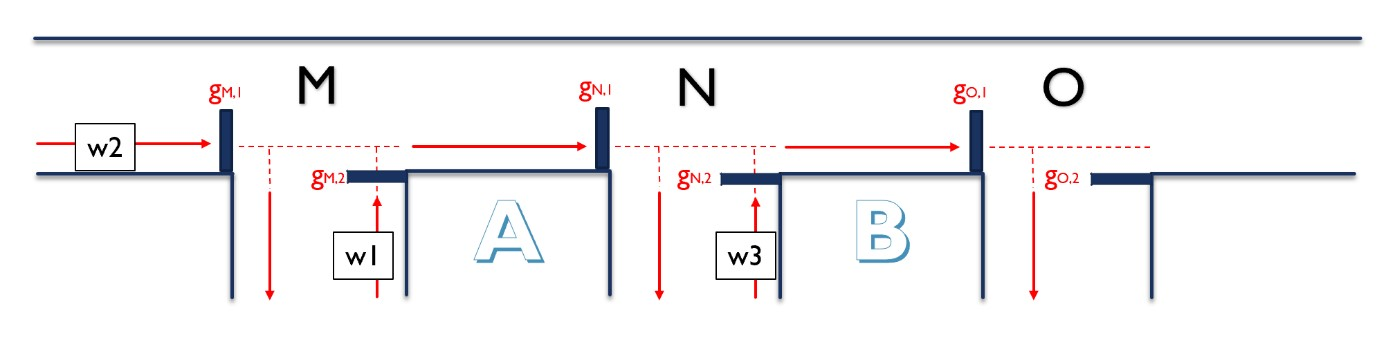
\includegraphics[width=15cm]{network-graph}
\end{figure}

\begin{figure}
    \caption{Network Graph}
      \centering
	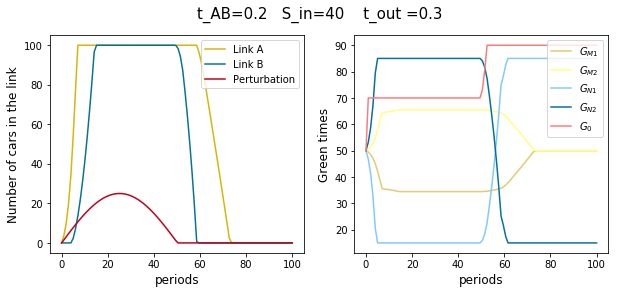
\includegraphics[width=15cm]{sim1}
\end{figure}

\begin{figure}
    \caption{Network Graph}
      \centering
	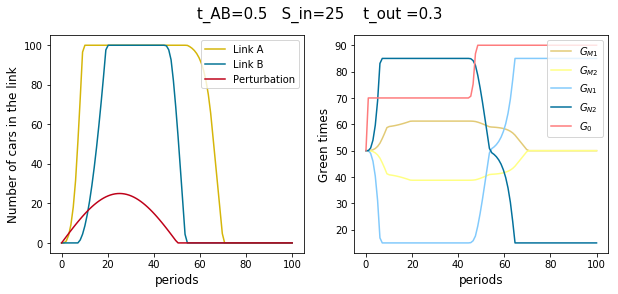
\includegraphics[width=15cm]{sim2}
\end{figure}

\begin{figure}
    \caption{Network Graph}
      \centering
	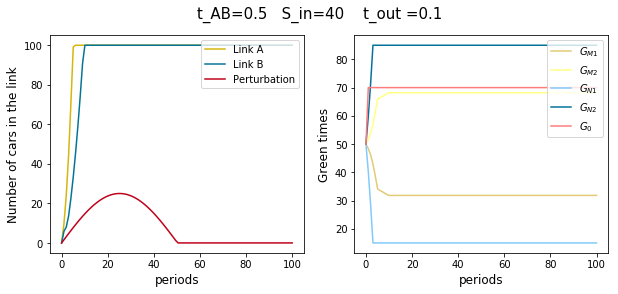
\includegraphics[width=15cm]{sim3}
\end{figure}

\begin{figure}
    \caption{Network Graph}
      \centering
	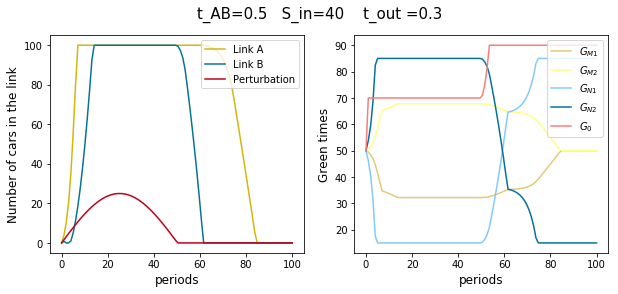
\includegraphics[width=15cm]{sim4}
\end{figure}

\begin{figure}
    \caption{Network Graph}
      \centering
	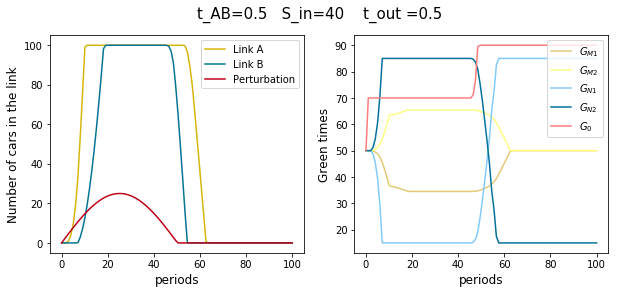
\includegraphics[width=15cm]{sim5}
\end{figure}

\begin{figure}
    \caption{Network Graph}
      \centering
	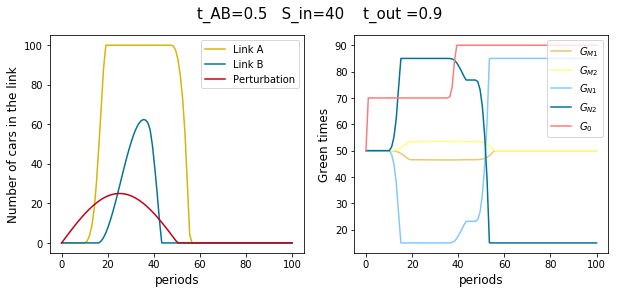
\includegraphics[width=15cm]{sim6}
\end{figure}

\begin{figure}
    \caption{Network Graph}
      \centering
	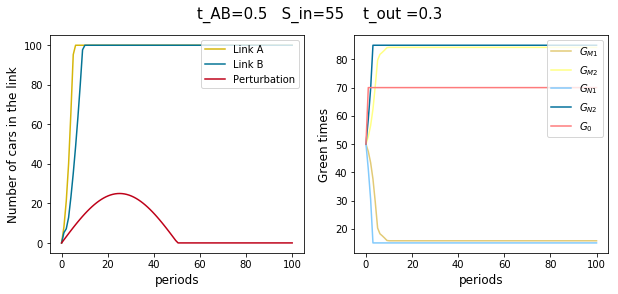
\includegraphics[width=15cm]{sim7}
\end{figure}

\begin{figure}
    \caption{Network Graph}
      \centering
	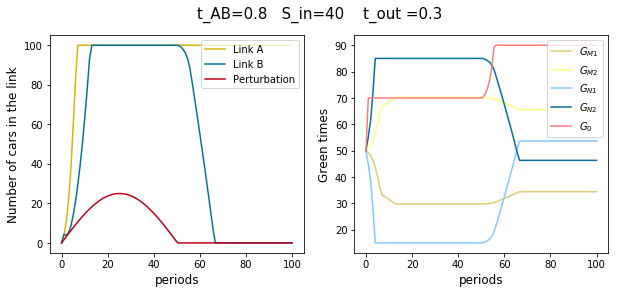
\includegraphics[width=15cm]{sim8}
\end{figure}

\section{Conclusion}

\begin{thebibliography}{9}
\bibitem{bertsekas} 
Bertsekas, D. (2005). Dynamic Programming and Optimal Control (3rd ed.). Athena Scientific.

\bibitem{diakaki1} 
Diakaki, C., Papageorgiou, M. \& Aboudolas, K. (2001).
A multivariable regulator approach to traffic-responsive network-wide signal control.
\textit{Control Engineering Practice} 10, 183-195.

\bibitem{diakaki2} 
Diakaki, C., Papageorgiou, M., \& McLean, T. (1997). Simulation studies of integrated corridor control in Glasgow. 
\textit{Transportation Research C}, 5, 211-224.

\end{thebibliography}

% ========== Continue adding items as needed

\end{document}
\grid
\grid